% !TEX program = pdflatex
\documentclass[12pt, a4paper]{article}

\usepackage[top=2.5cm, bottom=2.5cm, left=2.8cm, right=2.8cm]{geometry}
\usepackage{setspace}
\onehalfspacing
\usepackage{amsmath, amssymb}
\usepackage{graphicx}
\usepackage{booktabs}
\usepackage{multirow}
\usepackage{makecell}
\usepackage{float}
\usepackage{caption}
\captionsetup{font=small, labelfont=bf, skip=6pt}

\usepackage{listings}
\usepackage{xcolor}
\definecolor{codebg}{RGB}{248,248,248}
\definecolor{codeframe}{RGB}{200,200,200}
\definecolor{codekw}{RGB}{0,112,32}
\definecolor{codecomment}{RGB}{96,96,96}
\definecolor{codestr}{RGB}{186,33,33}
\lstset{
  backgroundcolor=\color{codebg},
  frame=single,
  rulecolor=\color{codeframe},
  basicstyle=\ttfamily\small,
  keywordstyle=\color{codekw}\bfseries,
  commentstyle=\color{codecomment}\itshape,
  stringstyle=\color{codestr},
  showstringspaces=false,
  breaklines=true,
  breakatwhitespace=true,
  tabsize=4,
  xleftmargin=1em,
  xrightmargin=0.5em,
  aboveskip=0.8em,
  belowskip=0.6em,
  numberstyle=\tiny\color{gray},
  numbers=left,
  numbersep=8pt,
}

\usepackage[hidelinks]{hyperref}
\usepackage[numbers, sort&compress]{natbib}

\newcommand{\intenttype}[1]{\texttt{#1}}
\newcommand{\filepath}[1]{\texttt{#1}}
\newcommand{\yang}{\textsc{YANG}}
\newcommand{\nsp}{\textsc{NSP}}
\newcommand{\lora}{\textsc{LoRA}}
\newcommand{\fillvalues}{\texttt{fill\_values}}

\usepackage{tikz}
\usetikzlibrary{arrows.meta, positioning, shapes.geometric, fit, calc}

\title{%
  \vspace{-1cm}
  {\LARGE\bfseries Automated Nokia NSP Network Service Intent\\[4pt]
  Generation via LoRA-Tuned Large Language Models}\\[12pt]
  {\large --- Personal Progress and Evaluation Report ---}
}
\author{%
  Wentao Sun \\[3pt]
  {\small\textit{Nokia Bell Labs}}
}
\date{\today}

\begin{document}
\maketitle
\thispagestyle{empty}

\begin{abstract}
\noindent
Nokia Network Services Platform (\nsp{}) is a widely deployed network service management platform in the telecommunications industry. Its core abstraction---the \emph{intent}---is a declarative JSON object that describes the desired state of a network service. Manually authoring intent JSON is challenging due to deep field paths, low fault tolerance, and high domain-knowledge requirements. This project fine-tuned Qwen3.5-9B with \lora{} (Low-Rank Adaptation) and implemented an end-to-end natural-language-to-intent pipeline for 9 NSP service intent types: epipe, tunnel, vprn, vpls, ies, etree, cpipe, evpn-epipe, and evpn-vpls. The system generates a compact \texttt{intent\_type + template\_name + fill\_values} object, expands it into NSP RESTCONF-shaped JSON, and validates it through a Nokia \yang{}-driven validation stack. The final adapter was trained on 2,640 generated training samples for 5 epochs and reaches 100\% on the primary held-out test metrics; the final golden-only regression run passes 11/11 hand-crafted cases.

\vspace{6pt}
\noindent\textbf{Keywords:} LLM fine-tuning, LoRA, network intent automation, Nokia NSP, YANG schema, structured output generation
\end{abstract}

\newpage
\tableofcontents
\newpage

\section{Introduction}

\subsection{Background}

Nokia \nsp{} is a unified network service orchestration platform for telecommunications operators. Its core work unit is the \emph{intent}---a declarative JSON configuration object that describes the desired state of a network service. Each intent consists of three core fields:

\begin{itemize}
  \item \textbf{intent\_type}: service type identifier (e.g., \intenttype{epipe}, \intenttype{vprn})
  \item \textbf{template\_name}: the corresponding \nsp{} template name
  \item \textbf{fill\_values}: a flat dictionary of dot-notation field paths mapped to \yang{} schema leaf nodes
\end{itemize}

\noindent
The \fillvalues{} field uses paths such as \texttt{site[0].interface[0].ipv4.primary.address}, corresponding to the hierarchical structure defined in the \yang{} schema. A typical multi-site VPRN configuration may contain 30--50 fields with path depths of 5--6 levels.

Manual authoring of \nsp{} intent JSON faces the following challenges:

\begin{enumerate}
  \item \textbf{High complexity}: deep field paths, large field counts, especially for multi-site services;
  \item \textbf{Low fault tolerance}: any path misspelling, type mismatch, or semantic conflict (e.g., missing SDP bidirectionality) results in deployment failure;
  \item \textbf{High knowledge barrier}: operators must simultaneously master \yang{} schema structures, \nsp{} API specifications, and service-specific network semantics.
\end{enumerate}

\subsection{Research Objective}

This project builds an end-to-end Natural Language to JSON (NL-to-JSON) automation system: operators describe network service requirements in natural language (e.g., ``Create an E-Pipe service from 192.168.0.16 to 192.168.0.37''), the model emits structured \fillvalues{}, and deterministic code expands the result into NSP RESTCONF-shaped intent JSON. Offline validation passing means the output is structurally consistent with the available \yang{} schemas and project semantic rules; live NSP server acceptance still requires future integration testing.

\subsection{Supported Intent Types}

The implemented system supports the 9 \nsp{} service intent types listed in Table~\ref{tab:intent-types}, covering L2/L3 VPN, MPLS tunneling, TDM emulation, and EVPN service categories.

\begin{table}[H]
\centering
\caption{Implemented 9 NSP intent types}
\label{tab:intent-types}
\small
\begin{tabular}{llll}
\toprule
\textbf{Intent Type} & \textbf{Service Category} & \textbf{Typical Scenario} & \textbf{Topology} \\
\midrule
\intenttype{epipe}       & L2 Point-to-Point & E-Line interconnect         & P2P \\
\intenttype{tunnel}      & MPLS Tunnel        & SDP tunnel establishment    & P2P \\
\intenttype{vprn}        & L3 VPN             & Multi-site IP-VPN           & Multipoint \\
\intenttype{vpls}        & L2 Multipoint      & Ethernet bridging domain    & Multipoint \\
\intenttype{ies}         & L3 Routed Access   & Internet Enhanced Service   & Single-site \\
\intenttype{etree}       & L2 Hub-Spoke       & Hub-spoke broadcast isolation & Tree \\
\intenttype{cpipe}       & TDM Emulation      & E1/T1 circuit emulation     & P2P \\
\intenttype{evpn-epipe}  & EVPN P2P           & BGP-controlled E-Line       & P2P \\
\intenttype{evpn-vpls}   & EVPN Multipoint    & BGP-controlled bridging     & Multipoint \\
\bottomrule
\end{tabular}
\end{table}

\section{Available Data Assets}
\label{sec:data-assets}

The project's data foundation comes from four authoritative sources, all organized and ready for training data construction.

\subsection{Nokia YANG Schemas}

We have obtained and organized the official Nokia \yang{} module files for all 9 intent types, stored under \filepath{data/yang/<intent\_type>/}. Parsing these schemas with the \texttt{pyang} library provides the following metadata for each field:

\begin{itemize}
  \item Canonical hierarchical path
  \item Base type (\texttt{int32}, \texttt{string}, \texttt{enumeration}, \texttt{boolean}, etc.)
  \item Value range constraints (e.g., \texttt{range "1..4094"} for VLAN IDs)
  \item String length constraints and regex patterns
  \item Enumeration value sets
  \item \texttt{mandatory}, \texttt{leaf-list}, \texttt{union} attributes
  \item List node key definitions and \texttt{min-elements}/\texttt{max-elements} constraints
\end{itemize}

\noindent
These schemas serve as the authoritative basis for both training data validation and model output verification.

\subsection{Nokia Canonical Payloads}

18 canonical JSON payload examples were extracted from the Nokia unified service management package (\texttt{nsp-service-mgmt-unified-25.8.3-rel.173.zip}). Their distribution is shown in Table~\ref{tab:canonical-payloads}.

\begin{table}[H]
\centering
\caption{Nokia canonical payload distribution}
\label{tab:canonical-payloads}
\small
\begin{tabular}{lcc}
\toprule
\textbf{Intent Type} & \textbf{Payload Count} & \textbf{Notes} \\
\midrule
\intenttype{vpls}        & 7 & Most comprehensive coverage \\
\intenttype{vprn}        & 3 & Variants with vastly different field counts \\
\intenttype{evpn-vpls}   & 3 & Covers mpls/vxlan/both modes \\
\intenttype{epipe}       & 2 & Basic dual-endpoint configurations \\
\intenttype{evpn-epipe}  & 2 & Covers mpls/vxlan modes \\
\intenttype{ies}         & 1 & Single-site routed access \\
\midrule
\intenttype{etree}       & 0 & No canonical payload in Nokia package \\
\intenttype{cpipe}       & 0 & No canonical payload in Nokia package \\
\intenttype{tunnel}      & 0 & No canonical payload in Nokia package \\
\bottomrule
\end{tabular}
\end{table}

\noindent
These payloads are used by the similarity-based reference validation tier (\S\ref{sec:tier6}). Note that 3 intent types have no canonical payloads, and existing payload field coverage varies significantly (e.g., vprn payloads range from $\sim$660 to $\sim$20 fields).

\subsection{Domain Knowledge Vocabulary}

We have compiled a domain knowledge vocabulary reflecting real Nokia operator environments:

\begin{itemize}
  \item \textbf{IP address ranges}: \texttt{10.x.x.x} management, \texttt{192.168.x.x} device interconnect
  \item \textbf{Port naming}: physical ports (\texttt{1/2/c4/1}) and LAG aggregates (\texttt{lag-\{vendor\}\{id\}-\{speed\}}, e.g., \texttt{lag-AFOR8-4x10GE})
  \item \textbf{Cluster name pool}: 35 Greek letter and celestial names
  \item \textbf{Project name pool}: 26 operator project names
  \item \textbf{Site descriptors}: 11 site role categories (datacenter, office, branch, pop, ...)
\end{itemize}

\subsection{Nokia Service Management Guide}

Chapters 4.7--4.19 of the Nokia Service Management Guide PDF provide parameter constraint descriptions and cross-field semantic rules for each service type, and were used to design and verify semantic validation rules.

\section{Technical Approach}
\label{sec:approach}

\subsection{Overall Architecture}

The current implementation contains a complete pipeline from data generation through model training, inference, merge, and validation. Figure~\ref{fig:pipeline} illustrates the system architecture.

\begin{figure}[H]
\centering
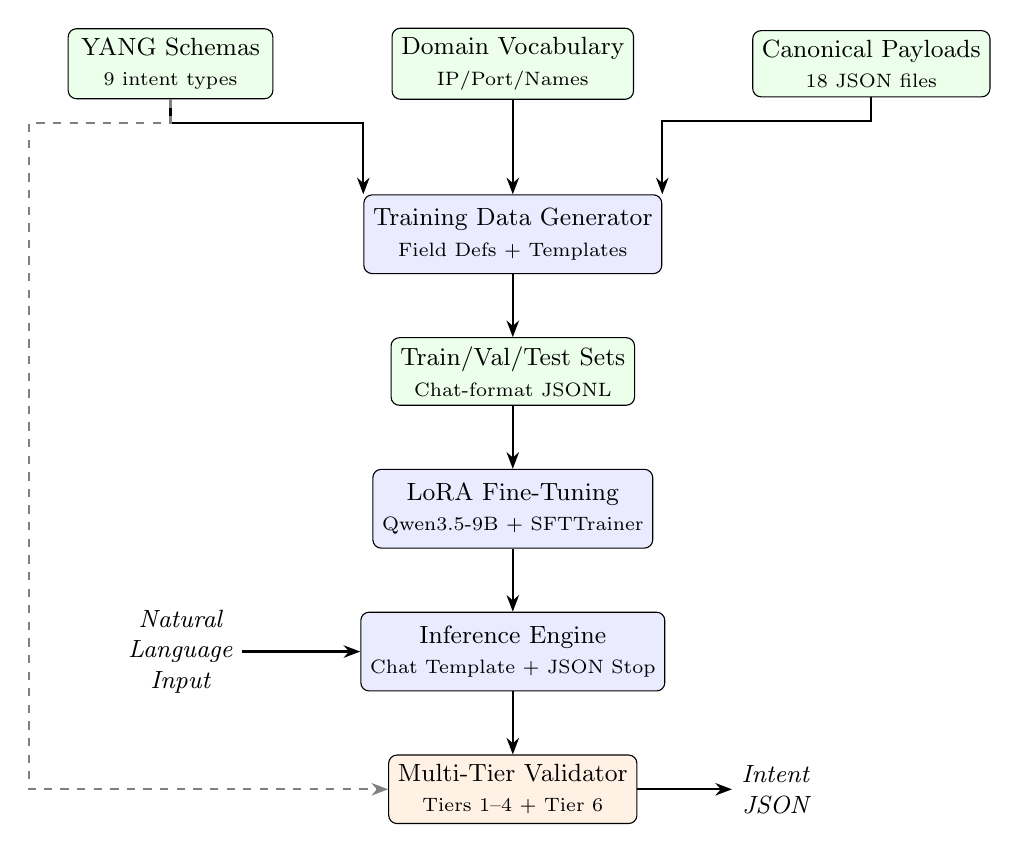
\begin{tikzpicture}[
  node distance=0.6cm and 1.2cm,
  every node/.style={font=\small},
  block/.style={rectangle, draw, rounded corners=3pt, minimum width=3.2cm, minimum height=1cm, fill=blue!8, align=center},
  data/.style={rectangle, draw, rounded corners=3pt, minimum width=2.6cm, minimum height=0.8cm, fill=green!8, align=center},
  valid/.style={rectangle, draw, rounded corners=3pt, minimum width=2.6cm, minimum height=0.8cm, fill=orange!10, align=center},
  arrow/.style={-{Stealth[length=6pt]}, thick},
]
  \node[data] (yang) {YANG Schemas\\{\scriptsize 9 intent types}};
  \node[data, right=1.5cm of yang] (vocab) {Domain Vocabulary\\{\scriptsize IP/Port/Names}};
  \node[data, right=1.5cm of vocab] (canon) {Canonical Payloads\\{\scriptsize 18 JSON files}};

  \node[block, below=1.2cm of vocab] (datagen) {Training Data Generator\\{\scriptsize Field Defs + Templates}};
  \node[data, below=0.8cm of datagen] (dataset) {Train/Val/Test Sets\\{\scriptsize Chat-format JSONL}};
  \node[block, below=0.8cm of dataset] (train) {LoRA Fine-Tuning\\{\scriptsize Qwen3.5-9B + SFTTrainer}};
  \node[block, below=0.8cm of train] (infer) {Inference Engine\\{\scriptsize Chat Template + JSON Stop}};
  \node[valid, below=0.8cm of infer] (validate) {Multi-Tier Validator\\{\scriptsize Tiers 1--4 + Tier 6}};

  \draw[arrow] (yang.south) -- ++(0,-0.3) -| (datagen.north west);
  \draw[arrow] (vocab.south) -- (datagen.north);
  \draw[arrow] (canon.south) -- ++(0,-0.3) -| (datagen.north east);
  \draw[arrow] (datagen) -- (dataset);
  \draw[arrow] (dataset) -- (train);
  \draw[arrow] (train) -- (infer);
  \draw[arrow] (infer) -- (validate);
  \draw[arrow, dashed, gray] (yang.south) -- ++(0,-0.3) -- ++(-1.8,0) |- (validate.west);

  \node[left=1.5cm of infer, align=center, font=\small\itshape] (nl) {Natural\\Language\\Input};
  \draw[arrow] (nl) -- (infer);

  \node[right=1.2cm of validate, align=center, font=\small\itshape] (out) {Intent\\JSON};
  \draw[arrow] (validate) -- (out);
\end{tikzpicture}
\caption{System architecture: end-to-end pipeline from data sources to validated output}
\label{fig:pipeline}
\end{figure}

\subsection{YANG Schema Parser}
\label{sec:yang-parser}

The schema parser serves as the system's data infrastructure. It uses the \texttt{pyang} library to parse Nokia's \yang{} modules and build a unified \texttt{SchemaIndex}. Core design decisions include:

\begin{enumerate}
  \item \textbf{Type chain resolution}: automatically trace \texttt{import}, \texttt{uses grouping}, and \texttt{typedef} chains, resolving derived types such as \texttt{inet:ipv4-address-no-zone} to their base \texttt{string} + \texttt{pattern} forms;
  \item \textbf{Dual-mode lookup}: support both exact path matching and suffix matching---the latter handles the project convention of omitting intermediate wrapper containers (e.g., \texttt{sdp-details.});
  \item \textbf{Envelope field handling}: \nsp{}'s envelope fields (\texttt{service-name}, \texttt{intent-type}, \texttt{olc-state}, etc.) are not defined in per-intent \yang{} modules and must be registered manually.
\end{enumerate}

\noindent
Each leaf node's metadata is encapsulated as:

\begin{lstlisting}[language=Python, caption={LeafMeta data structure}]
@dataclass
class LeafMeta:
    path: str               # Canonical YANG path
    base_type: str          # Base type (int32/string/boolean/...)
    range_expr: str | None  # Value range constraint
    length_expr: str | None # String length constraint
    pattern_list: list[str] # Regex patterns
    enum_values: list[str]  # Enumeration value set
    mandatory: bool         # Whether mandatory
    is_leaf_list: bool      # leaf-list flag
    union_types: list       # Union member types
\end{lstlisting}

\subsection{Multi-Tier Validation Framework}
\label{sec:validation}

The validation framework is the core quality assurance mechanism. It implements a five-tier progressive validation stack as illustrated in Figure~\ref{fig:validation-tiers}.

\begin{figure}[H]
\centering
\resizebox{\textwidth}{!}{%
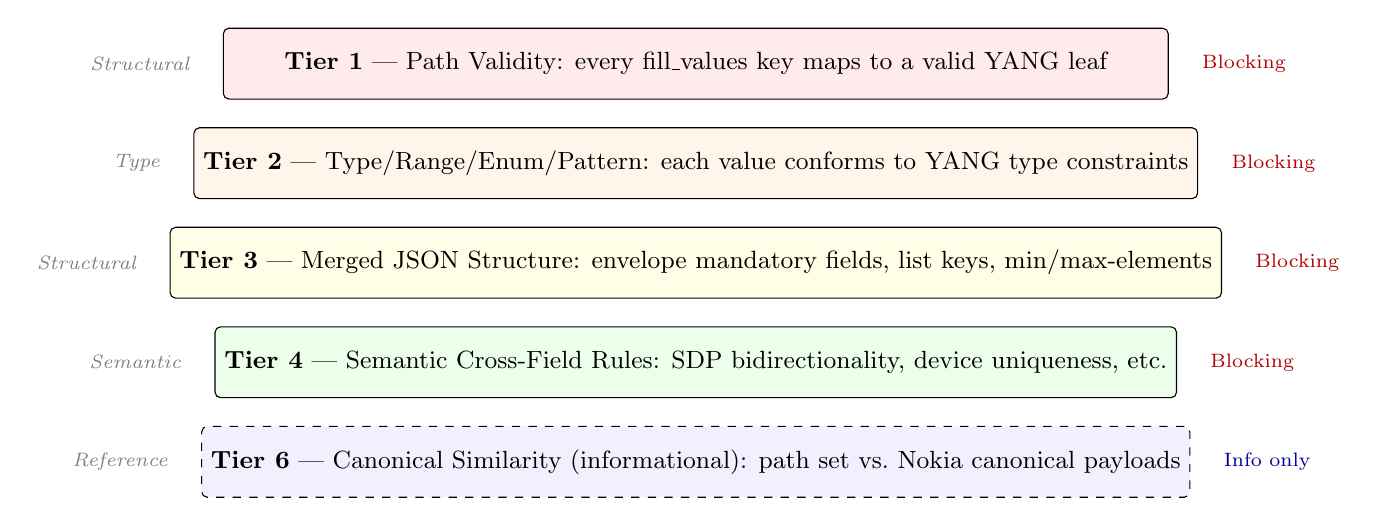
\begin{tikzpicture}[
  every node/.style={font=\small},
  tier/.style={rectangle, draw, rounded corners=2pt, minimum width=12cm, minimum height=0.9cm, align=center},
  node distance=0.35cm,
]
  \node[tier, fill=red!8]    (t1) {\textbf{Tier 1} --- Path Validity: every fill\_values key maps to a valid YANG leaf};
  \node[tier, fill=orange!8, below=of t1] (t2) {\textbf{Tier 2} --- Type/Range/Enum/Pattern: each value conforms to YANG type constraints};
  \node[tier, fill=yellow!10, below=of t2] (t3) {\textbf{Tier 3} --- Merged JSON Structure: envelope mandatory fields, list keys, min/max-elements};
  \node[tier, fill=green!8,  below=of t3] (t4) {\textbf{Tier 4} --- Semantic Cross-Field Rules: SDP bidirectionality, device uniqueness, etc.};
  \node[tier, fill=blue!6, dashed, below=of t4] (t6) {\textbf{Tier 6} --- Canonical Similarity (informational): path set vs.\ Nokia canonical payloads};

  \node[left=0.3cm of t1, font=\scriptsize\itshape, text=gray] {Structural};
  \node[left=0.3cm of t2, font=\scriptsize\itshape, text=gray] {Type};
  \node[left=0.3cm of t3, font=\scriptsize\itshape, text=gray] {Structural};
  \node[left=0.3cm of t4, font=\scriptsize\itshape, text=gray] {Semantic};
  \node[left=0.3cm of t6, font=\scriptsize\itshape, text=gray] {Reference};

  \node[right=0.3cm of t1, font=\scriptsize, text=red!70!black] {Blocking};
  \node[right=0.3cm of t2, font=\scriptsize, text=red!70!black] {Blocking};
  \node[right=0.3cm of t3, font=\scriptsize, text=red!70!black] {Blocking};
  \node[right=0.3cm of t4, font=\scriptsize, text=red!70!black] {Blocking};
  \node[right=0.3cm of t6, font=\scriptsize, text=blue!60!black] {Info only};
\end{tikzpicture}%
}
\caption{Five-tier progressive validation stack}
\label{fig:validation-tiers}
\end{figure}

\subsubsection{Tier 1: Path Validity}

Verifies that every key in \fillvalues{} corresponds to a valid leaf path in the \yang{} schema. The \texttt{SchemaIndex} uses suffix matching to handle abbreviated paths. For example, \texttt{sdp[0].sdp-id} is correctly identified even though its full \yang{} path is \texttt{epipe.sdp-details.sdp[0].sdp-id}.

\subsubsection{Tier 2: Type/Range/Enum/Pattern}

Performs type validation on each value:

\begin{itemize}
  \item \textbf{Integer types} (int8--int64, uint8--uint64): check base type bounds and \yang{} \texttt{range} expressions
  \item \textbf{String types}: check \texttt{length} constraints and \texttt{pattern} regexes
  \item \textbf{Enumeration types}: verify the value belongs to the valid enumeration set
  \item \textbf{Union types}: try each member type; at least one must match
  \item \textbf{Boolean types}: accept Python \texttt{bool} and string representations
\end{itemize}

\subsubsection{Tier 3: Merged JSON Structural Validation}

Runs after \fillvalues{} is merged into the full intent JSON, checking:

\begin{itemize}
  \item Root key \texttt{nsp-service-intent:intent} array exists and is non-empty
  \item Envelope mandatory fields are populated (e.g., tunnel's \texttt{name/source-ne-id/sdp-id})
  \item All \yang{} list entry key fields are present
  \item List entry counts satisfy \texttt{max-elements}/\texttt{min-elements} constraints
\end{itemize}

\subsubsection{Tier 4: Semantic Cross-Field Rules}

Validates cross-field constraints that \yang{} schemas cannot express. Table~\ref{tab:semantic-rules} lists the implemented semantic rules for each intent type.

\begin{table}[H]
\centering
\caption{Tier 4 semantic rules per intent type}
\label{tab:semantic-rules}
\small
\begin{tabular}{lp{9cm}}
\toprule
\textbf{Intent Type} & \textbf{Semantic Rules} \\
\midrule
\intenttype{epipe} &
  SDP bidirectionality; VLAN tags match; devices differ \\
\intenttype{tunnel} &
  source-ne-id $\neq$ destination-ne-id \\
\intenttype{vprn} &
  All site device-ids distinct; RD format \texttt{ASN:ID} \\
\intenttype{vpls} / \intenttype{evpn-vpls} &
  Site device-ids distinct; outer VLAN tags consistent \\
\intenttype{etree} &
  $\geq$1 root + $\geq$1 leaf SAP; device-ids distinct \\
\intenttype{ies} &
  Only site[0] allowed; no extra sites permitted \\
\intenttype{cpipe} &
  Devices differ; time-slots match; vc-type in valid enum \\
\intenttype{evpn-epipe} &
  evpn-type matches sub-tree (mpls/vxlan); eth-tag = VLAN \\
\bottomrule
\end{tabular}
\end{table}

\subsubsection{Tier 6: Canonical Payload Similarity}
\label{sec:tier6}

Compares the model output's path set against Nokia canonical payload path sets. Path normalization includes stripping wrapper containers (e.g., \texttt{*-details.}) and folding list indices to wildcards (\texttt{site[0]} $\to$ \texttt{site[*]}). This tier is informational and non-blocking, since the canonical payloads themselves are incomplete---3 intent types have no canonical payloads at all.

\section{Current Progress}

\subsection{Implementation Status}

The repository now contains the full pipeline:

\begin{itemize}
  \item \textbf{Data generation}: \filepath{data/generate\_training\_data.py}, \filepath{data/field\_definitions.py}, and \filepath{data/instruction\_templates.py} generate 3,300 synthetic train/validation/test samples plus 11 golden tests.
  \item \textbf{Schema and validation}: \filepath{data/yang\_schema.py} parses Nokia \yang{} modules; \filepath{data/intent\_validator.py} implements Tier 1+2, Tier 3, Tier 4, and Tier 6 checks.
  \item \textbf{Training}: \filepath{train/train\_qwen3\_nsp.py} trains Qwen3.5-9B with LoRA (r=32, alpha=64, BF16, two-GPU DDP, max length 8192).
  \item \textbf{Inference}: \filepath{inference/predict.py} loads the base model and LoRA adapter, applies Qwen chat-template alignment with \texttt{enable\_thinking=False}, extracts JSON, merges \fillvalues{}, and runs validation.
  \item \textbf{Demo}: \filepath{demos/demo\_all\_types.py} runs one live example for each of the 9 intent types and saves merged JSON under \filepath{demos/output/}.
\end{itemize}

\subsection{Data Sources}

The training and validation design uses four data sources:

\begin{itemize}
  \item \textbf{Nokia \yang{} modules}: stored under \filepath{data/yang/}, covering all 9 service intent types.
  \item \textbf{Canonical payload examples}: 18 Nokia-shipped JSON payloads under \filepath{data/canonical\_payloads/}, covering epipe, vprn, vpls, ies, evpn-epipe, and evpn-vpls.
  \item \textbf{Reference artifacts}: Nokia NSP 25.8 service-management packages and PDFs under \filepath{references/}.
  \item \textbf{Domain vocabulary}: IP ranges, Nokia-style port names, project names, cluster names, route distinguishers, and topology conventions in \filepath{data/value\_generators.py}.
\end{itemize}

\subsection{Training and Evaluation Results}

The final adapter is stored under \filepath{output/qwen3-nsp-intent-adapter/}. It was trained for 5 epochs on 2,640 training samples. The latest complete evaluation run reports the following test-set metrics:

\begin{table}[H]
\centering
\caption{Final evaluation summary}
\small
\begin{tabular}{lcc}
\toprule
\textbf{Metric} & \textbf{Test set (330)} & \textbf{Golden tests (11)} \\
\midrule
JSON Valid Rate & 100.0\% & 100.0\% \\
Intent Type Accuracy & 100.0\% & 100.0\% \\
Field Recall & 100.0\% & 100.0\% \\
Field Precision & 100.0\% & 100.0\% \\
Value Accuracy & 100.0\% & 100.0\% \\
Tier 1--4 Valid & 100.0\% & 100.0\% \\
Tier 6 Canonical Recognition & 96.6\% & informational \\
\bottomrule
\end{tabular}
\end{table}

\noindent
The test-set values come from \filepath{output/logs/m3\_5final\_eval.log}. The final golden pass count comes from the later golden-only regression log, \filepath{output/logs/golden\_only\_eval.log}.

\subsection{Important Limitations}

\begin{enumerate}
  \item \textbf{Offline validation is a structural lower bound}: Tier 1--4 passing means the generated JSON is consistent with available \yang{} schema and project semantic checks. NSP's server-side JavaScript mapping engine may still reject an intent.
  \item \textbf{Test data is generated from the same distribution as training data}: out-of-distribution operator phrasing and real NSP deployment acceptance remain future work.
  \item \textbf{Canonical payload coverage is incomplete}: etree, cpipe, and tunnel have no Nokia canonical payloads in the available package, so Tier 6 cannot score those types.
\end{enumerate}

\end{document}
